\documentclass{standalone}
\usepackage{tikz}
\usepackage{pgfplots}
\pgfplotsset{width=32cm,height=18cm,compat=1.3}
\pgfplotsset{every tick label/.append style={font=\Huge}}
\usepackage{filecontents}

\usetikzlibrary{patterns}

\definecolor{citrine}{rgb}{0.89, 0.82, 0.04}

\begin{document}
	\centering
		\vspace{1.5em}
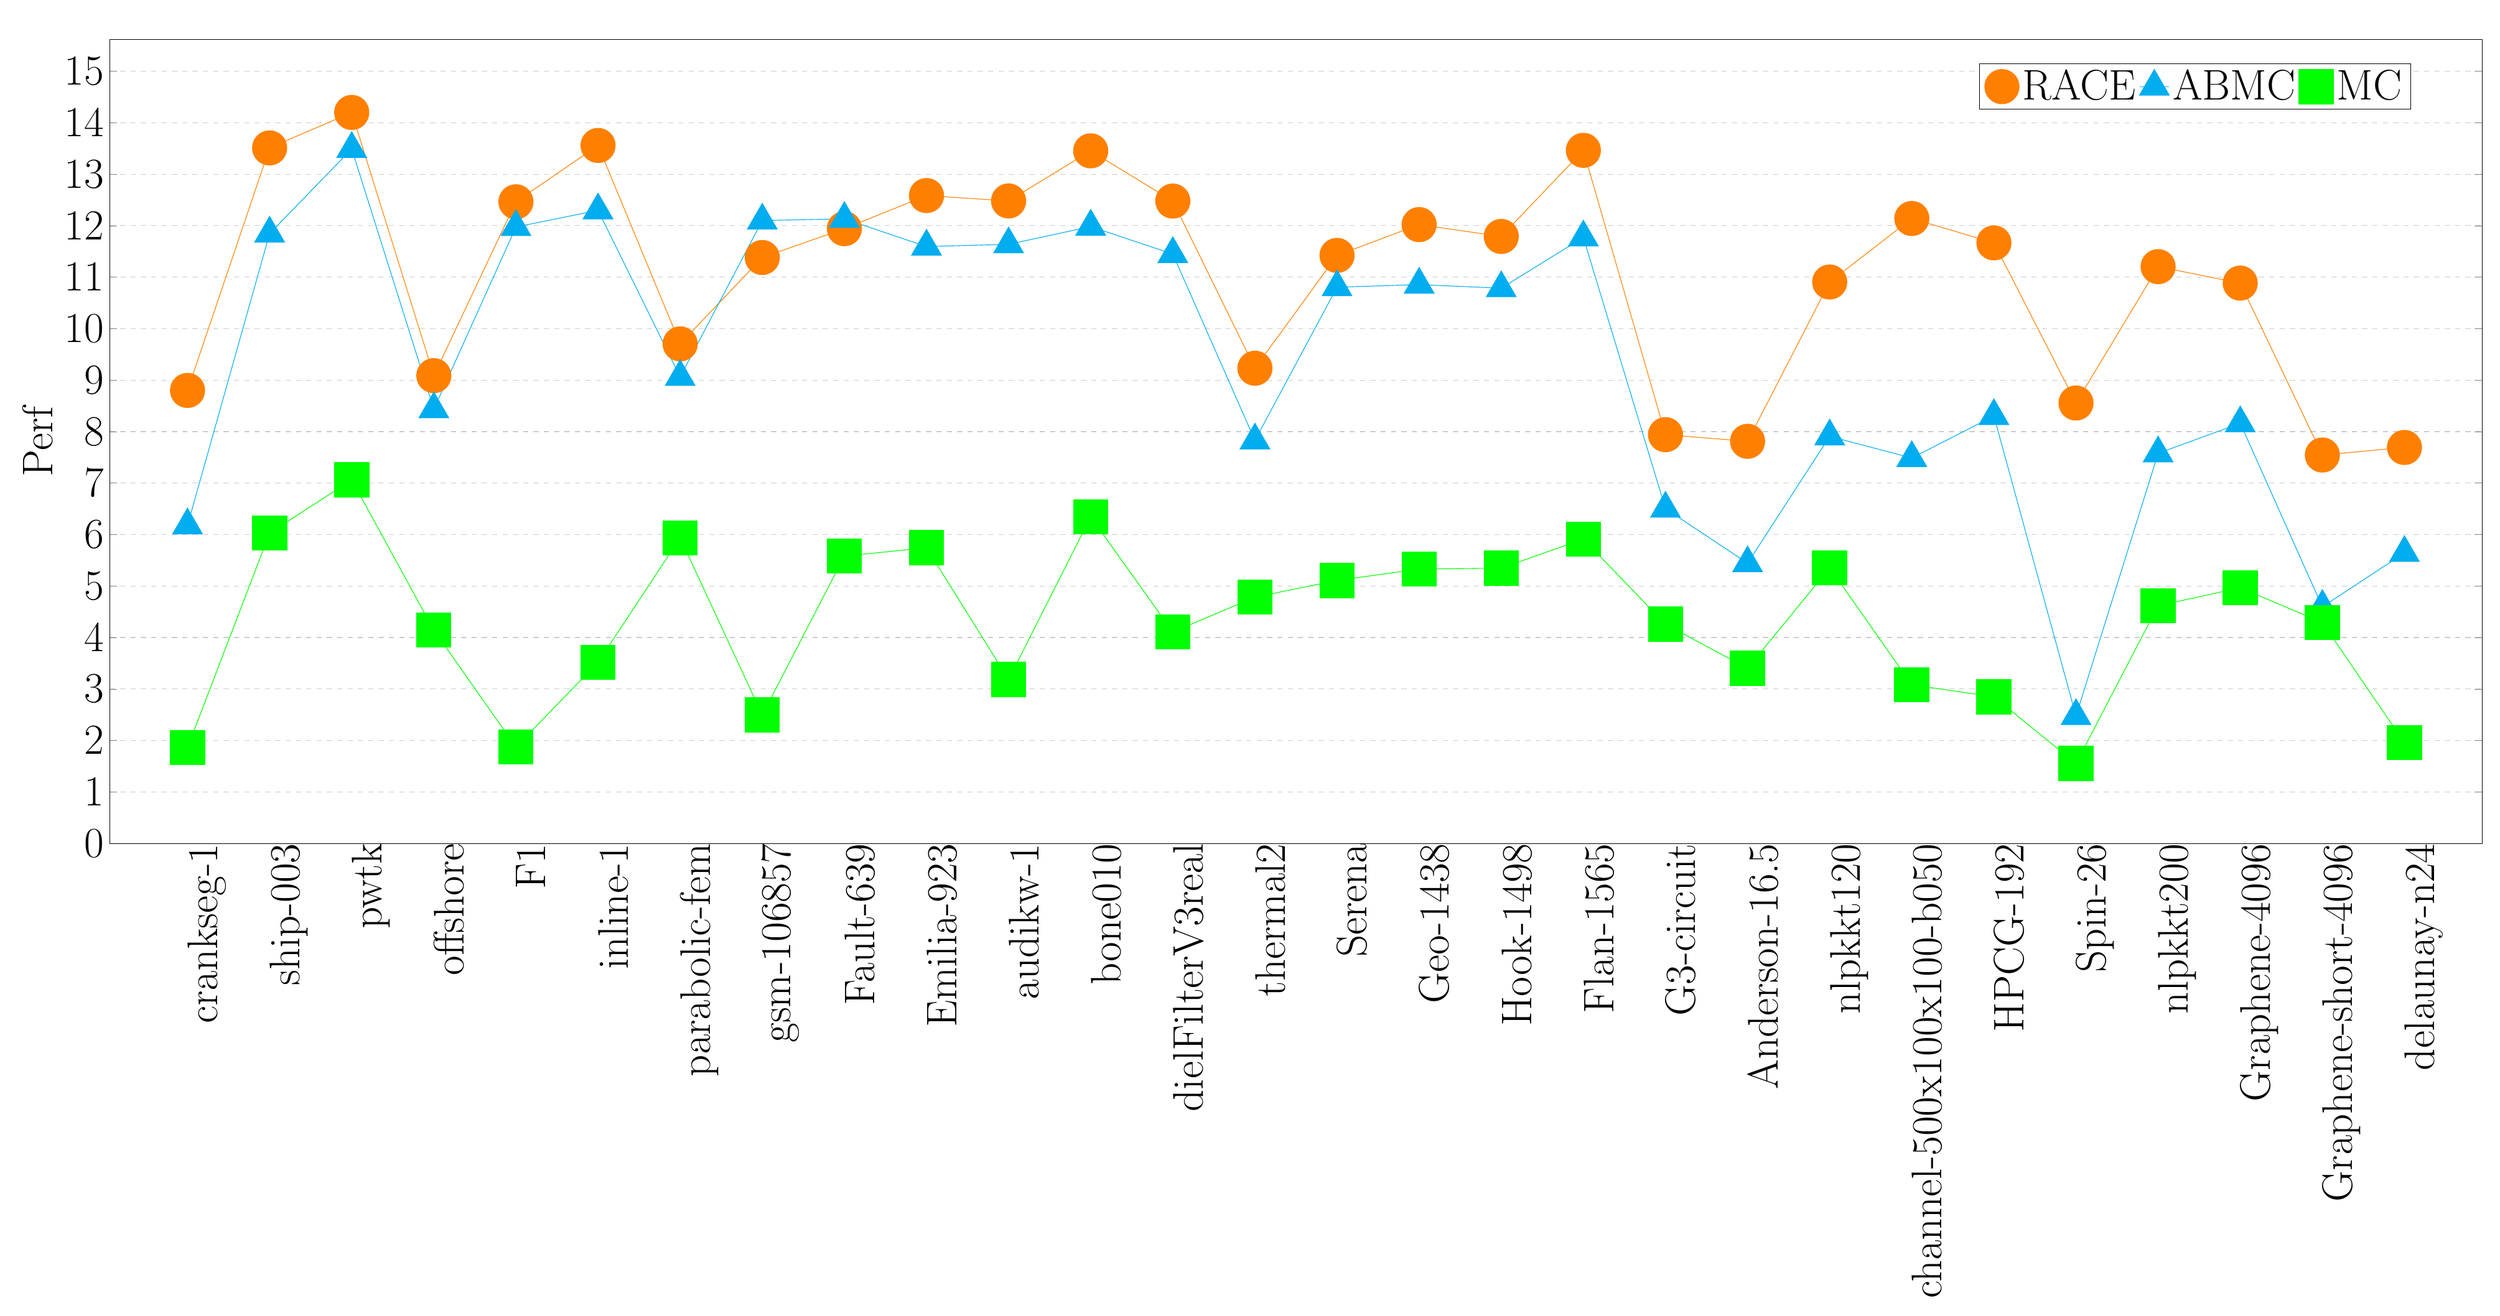
\begin{tikzpicture}
		%	\node at (13.25,15) {\LARGE{}};
			\begin{axis}[
		%	xmin=0.25, xmax=7.25,
			ymin=0, %ymax=3.25,
			xtick={1, 2, 3, 4, 5, 6, 7, 8, 9, 10, 11, 12, 13, 14, 15, 16, 17, 18, 19, 20, 21, 22, 23, 24, 25, 26, 27, 28},
		%	ytick={0,0.5,1,1.5,2,2.5,3},
			xticklabels={crankseg-1, ship-003, pwtk, offshore, F1, inline-1, parabolic-fem, gsm-106857, Fault-639, Emilia-923, audikw-1, bone010, dielFilterV3real, thermal2, Serena, Geo-1438, Hook-1498, Flan-1565, G3-circuit, Anderson-16.5, nlpkkt120, channel-500x100x100-b050, HPCG-192, Spin-26, nlpkkt200, Graphene-4096, Graphene-short-4096, delaunay-n24},
			width  = 50cm,
			height = 18cm,
			major x tick style = transparent,
			%	minor ytick={1, 5, 10, 15, 20, 25, 30 ,35,40},
			grid = minor,	
			%add_bar_commands
			ymajorgrids = true,
			grid style={dashed, gray!40},
			ylabel = {\Huge{Perf}},
		%	symbolic x coords={Graphene-2048-2048, Graphene-4096-4096, Spin-24-24-24},
			x tick label style={rotate=90, anchor=north east, inner sep=0mm, font={\Huge}},
			tick label style={font={\Huge}},
			scaled y ticks = false,
			enlarge x limits=0.035,
			legend cell align=left,
			legend style={font=\Huge},
			legend columns=-1,
			legend style={
				%at={(1,1.05)},
				%anchor=south east,
				%column sep=1ex,
				legend pos=north east
			},
			%spl_legend_code
			title= {\Huge\scalebox{1.5}{{}}}
			]

\addplot[mark=*, mark size=10pt, mark options={orange}, draw=orange ] plot coordinates{(1,8.799993) (2,13.511751) (3,14.200478) (4,9.087057) (5,12.464941) (6,13.559009) (7,9.703977) (8,11.382424) (9,11.942039) (10,12.585517) (11,12.481031) (12,13.454827) (13,12.478694) (14,9.231351) (15,11.422656) (16,12.021507) (17,11.791030) (18,13.463977) (19,7.939802) (20,7.811229) (21,10.906182) (22,12.139824) (23,11.666773) (24,8.555170) (25,11.204207) (26,10.884372) (27,7.545134) (28,7.691780)};
\addplot[mark=triangle*, mark size=10pt, mark options={cyan}, draw=cyan ] plot coordinates{(1,6.178656) (2,11.847884) (3,13.491702) (4,8.435306) (5,11.974533) (6,12.298856) (7,9.062039) (8,12.100507) (9,12.132818) (10,11.595278) (11,11.638545) (12,11.982375) (13,11.449803) (14,7.829024) (15,10.805083) (16,10.855085) (17,10.786634) (18,11.772924) (19,6.503159) (20,5.443401) (21,7.907156) (22,7.487216) (23,8.302103) (24,2.473984) (25,7.577819) (26,8.162013) (27,4.595417) (28,5.642745)};
\addplot[mark=square*, mark size=10pt, mark options={green}, draw=green ] plot coordinates{(1,1.861477) (2,6.027780) (3,7.061438) (4,4.143928) (5,1.871931) (6,3.517903) (7,5.934224) (8,2.495243) (9,5.580948) (10,5.743727) (11,3.184375) (12,6.343043) (13,4.107050) (14,4.783377) (15,5.108226) (16,5.329090) (17,5.347373) (18,5.911824) (19,4.257442) (20,3.400937) (21,5.354115) (22,3.080497) (23,2.847961) (24,1.552193) (25,4.616286) (26,4.966167) (27,4.290495) (28,1.956021)};
	%addplot cmd

	\legend{RACE, ABMC, MC}

	\end{axis}			
\end{tikzpicture}

\end{document}

